\documentclass[10pt]{report}
\usepackage[spanish]{babel}
\usepackage[utf8]{inputenc}
\usepackage{amsmath,amsthm,amsfonts,amssymb}
\usepackage{Sweave}
\usepackage{graphicx}
\usepackage{hyperref}
\usepackage{anysize} 
\usepackage{lscape}
\usepackage{multirow} % para las tablas
\marginsize{1.5cm}{1.5cm}{0.5cm}{0.5cm} 

\title{\Huge Universidad Nacional de Loja \\ 
Área de la Energía las Industrias y los Recursos Naturales no Renovables \\
Ingeniería en Sistemas \\}

\author{
\includegraphics[width=6cm, height=6cm]{unloja.png}\\\\   
  JOHANNA ESTEFANIA PAZ JIMENEZ \\ ECINF7330\\  \texttt{johanna.paz@unl.edu.ec}\\ \\
}

\begin{document}
\Sconcordance{concordance:1105652190.tex:1105652190.Rnw:%
1 48 1 1 2 34 0 1 2 3 1 1 5 11 0 1 2 2 1 1 3 5 0 1 2 1 1 1 2 3 0 1 2 3 %
0 1 2 2 0 1 2 4 0 1 2 1 1 1 4 1 2 3 1}

\maketitle
\begin{center}\textbf{\Large SWEBOK}\end{center}

\textbf{Descripción}\\

La (aproximadamente) calificación trimestral aprobación para el Presidente de los Estados Unidos a partir del primer trimestre de 1945 hasta el último trimestre de 1.974.\\

\textbf{Uso}\\

Presidents.\\

\textbf{Formato}\\

Una serie de tiempo de 120 valores.\\


\textbf{Detalles}

Los datos son en realidad una versión amañadas de los índices de aprobación. Ver el libro de McNeil para más detalles.\\

\textbf{Fuente}\\

McNeil, D. R. (1977) Interactive Data Analysis. New York: Wiley\\

%\textbf{Determinar la estadística, cuando presidents son mayores a 1900}\\

\textbf{Tabla:}\\
\begin{Schunk}
\begin{Soutput}
     Qtr1 Qtr2 Qtr3 Qtr4
1945   NA   87   82   75
1946   63   50   43   32
1947   35   60   54   55
1948   36   39   NA   NA
1949   69   57   57   51
1950   45   37   46   39
1951   36   24   32   23
1952   25   32   NA   32
1953   59   74   75   60
1954   71   61   71   57
1955   71   68   79   73
1956   76   71   67   75
1957   79   62   63   57
1958   60   49   48   52
1959   57   62   61   66
1960   71   62   61   57
1961   72   83   71   78
1962   79   71   62   74
1963   76   64   62   57
1964   80   73   69   69
1965   71   64   69   62
1966   63   46   56   44
1967   44   52   38   46
1968   36   49   35   44
1969   59   65   65   56
1970   66   53   61   52
1971   51   48   54   49
1972   49   61   NA   NA
1973   68   44   40   27
1974   28   25   24   24
\end{Soutput}
\end{Schunk}

\textbf{Determinar la estadística, cuando presidents son mayores a 1950 y menores a 1970}\\
% todos los presidentes son mayores a 1900
%x <- cbind(x, 12)
\begin{Schunk}
\begin{Soutput}
       V1              V2              V3              V4       
 Min.   :25.00   Min.   :24.00   Min.   :32.00   Min.   :23.00  
 1st Qu.:58.00   1st Qu.:50.50   1st Qu.:57.25   1st Qu.:49.00  
 Median :71.00   Median :62.00   Median :62.50   Median :57.00  
 Mean   :62.37   Mean   :59.58   Mean   :60.22   Mean   :56.95  
 3rd Qu.:74.00   3rd Qu.:69.50   3rd Qu.:69.00   3rd Qu.:67.50  
 Max.   :80.00   Max.   :83.00   Max.   :79.00   Max.   :78.00  
                                 NA's   :1                      
\end{Soutput}
\end{Schunk}

\textbf{Determinar la estadística, cuando Qtr2 son menores a 70 y mayores a 50, Cuál es el 3erQ?}\\
%a <- (x[,2] < 70 & x[,2] > 50)
\begin{Schunk}
\begin{Soutput}
   Min. 1st Qu.  Median    Mean 3rd Qu.    Max. 
  24.00   48.25   60.50   56.43   64.75   87.00 
\end{Soutput}
\end{Schunk}

\textbf{Determinar la estadística, cuando Qtr1 y Qtr4 están asignación (NA)}\\
\begin{Schunk}
\begin{Soutput}
[1] "Estadistico_de_Qtr1"
\end{Soutput}
\begin{Soutput}
   Min. 1st Qu.  Median    Mean 3rd Qu.    Max.    NA's 
  25.00   45.00   63.00   58.45   71.00   80.00       1 
\end{Soutput}
\begin{Soutput}
[1] "Estadistico_de_Qtr4"
\end{Soutput}
\begin{Soutput}
   Min. 1st Qu.  Median    Mean 3rd Qu.    Max.    NA's 
  23.00   44.00   55.50   53.07   63.00   78.00       2 
\end{Soutput}
\end{Schunk}

\textbf{Graficar Qtr1 Vs Qtr2, cuando Qtr1 no tiene asignación.}\\
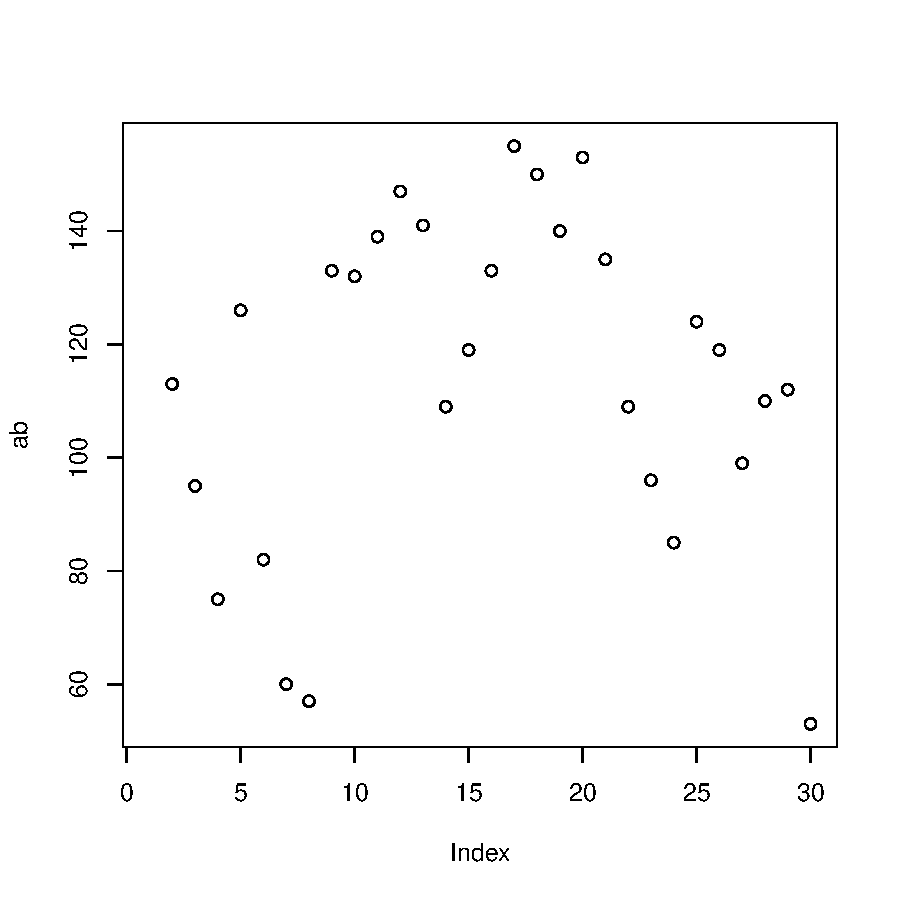
\includegraphics{1105652190-005}
\begin{center}
%\includegraphics[width=6cm, height=1.5cm]{cc.jpg}
\end{center}
\end{document}
